% !TeX root = ../main.tex

\chapter{工作负载}

\section{TPC-C基准测试集}
TPC-C\cite{TPCC}是由事务处理性能委员会所制定的标准测试之一,被用来测试事务处理系统的性能。其模拟了一个大型的商业环境,具有一定的商务仿真性,因此其测试结果对于设计高性能的事务处理系统具有一定的指导意义。

具体来说,TPCC模拟了大型的批发销售公司,该公司在多个区域有业务,并且使用仓库管理。当公司商务拓展时,就有新的仓库加入管理。每个仓库负责10个区域的供货,每个区域服务3000个客户,并且每个仓库维护100000个商品的库存信息。其垂直结构如下图所示:

\begin{figure}[htb]
  \centering
  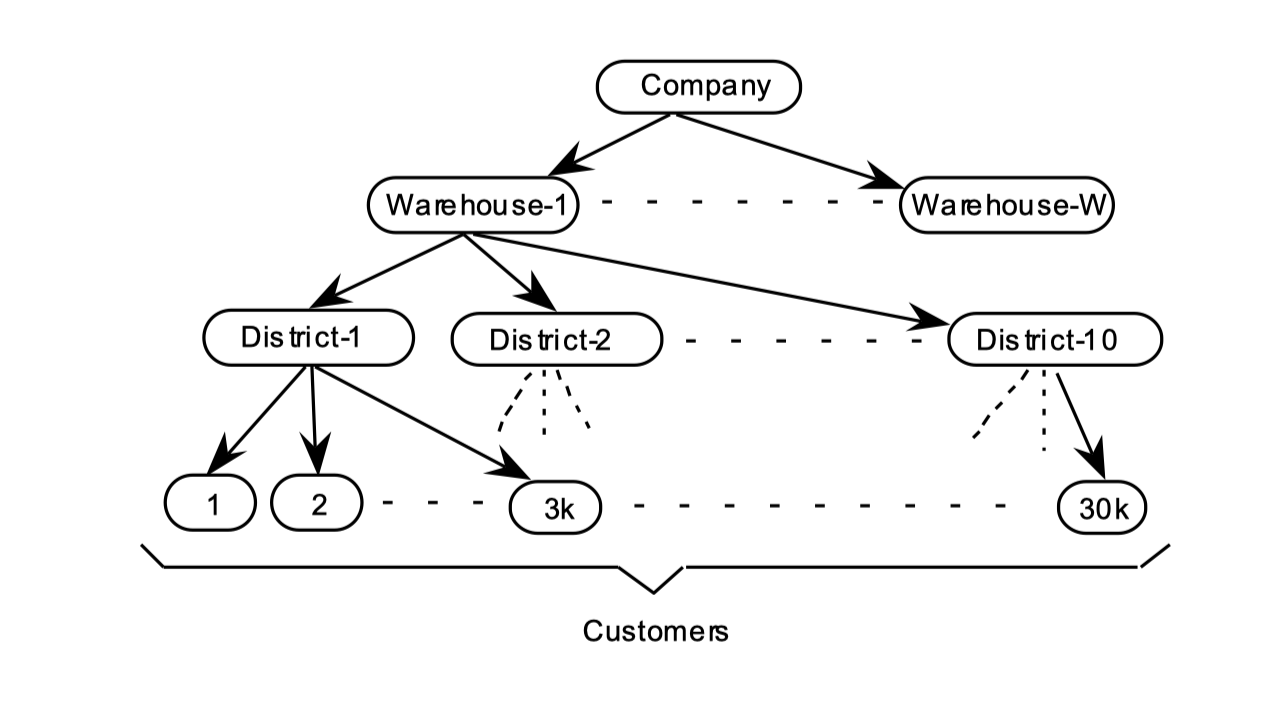
\includegraphics[width=0.8\textwidth]{TPCC-1.png}
  \caption{分层设计模型}
  \label{fig:badge}
\end{figure}

TPCC由9个表格组成,他们各自的依赖关系如下:

\begin{figure}[htb]
  \centering
  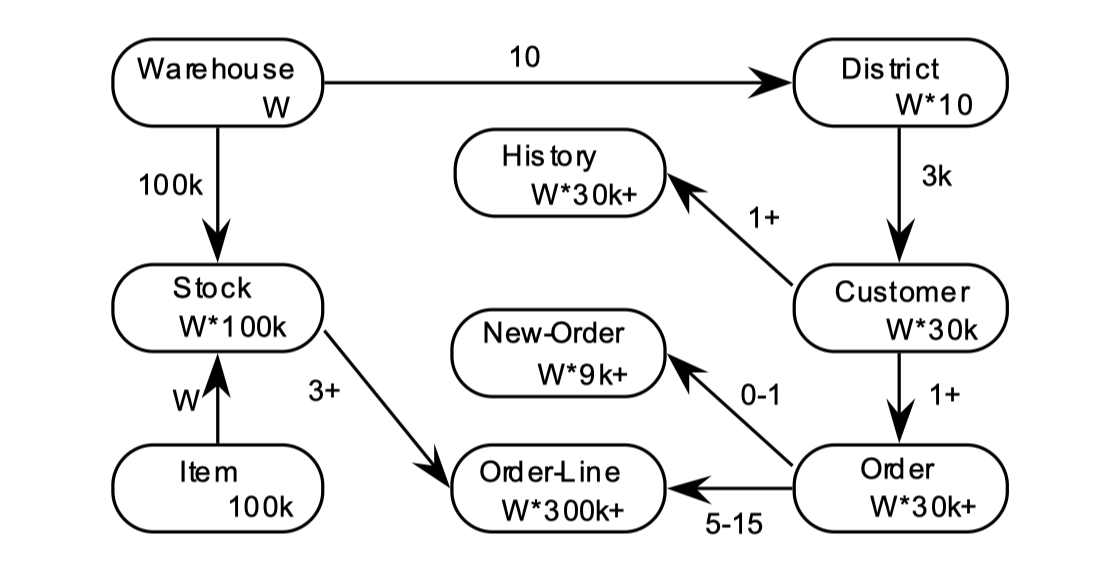
\includegraphics[width=0.8\textwidth]{TPCC-2.png}
  \caption{分层设计模型}
  \label{fig:badge}
\end{figure}

\subsection{TPC-C基本特征分析}
我们使用TPC-C来衡量异地冗余存储系统的事务处理性能,因此我们就需要分析TPC-C事务的访问模型,跨数据中心的事务所占的比例,单数据中心事务所占的比例。每个事务访问的表格有哪些等等。根据TPC-C 5.11.0标准,归纳如下:

(1)New Order:用户用于订购5-15件商品,约有1\%订购的商品不存在,此时需要放弃事务的提交。并且有1\%订购的商品来自于远程仓库,即存在跨数据中心的订单请求。用户订购的商品以及供应的仓库随机生成。

(2)Payment:用户使用账户余额支付订购的账单。约有40\%的事务请求,根据用户的id发出,另外60\%的订单根据用户的名字生成。并且有15\%的事务用户与供货仓库不在一个数据中心内,也就是说此事用户需要跨数据中心支付。

(3)Order Status:用于查询最近的一个订单状态,与Payment 事务类似,约有40\%的事务请求,根据用户的id发出,另外60\%的订单根据用户的名字生成。事务首先根据用户信息得到最新的订单号,在根据订单号查询订单信息。

(4)Delivery:为一个仓库的每个区域中的新订单(尚未被指派拌匀者的订单)中排序最前的指派搬运者。事务首先收集订单号较小的新订单的订单号,再为这些订单指派搬运者。

(5)Stock Level:查询最近被订购的商品的库存水品,事务首先取得最近订购商品的订单号,再根据订单号到订单发生的仓库查询库存情况。因此该事务存在跨数据中心的查询。
\\
\begin{table}[htb]
  \centering\small
  \caption{TPC-C各个事务涉及的表格极其访问模式}
  \label{tab:exampletable}
  \begin{tabular}{p{90pt}p{160pt}p{130pt}}
    \toprule
    事务类型   & 涉及的表格 & 访问模式 \\
    \midrule
    New Order & warehouse、district、customer、order、new order、item、stock、order line  & 存在跨数据中心访问 \\
    Payment & warehouse、district、customer、history & 存在跨数据中心访问  \\
    Order Status &  customer、order、order line & 不存在跨数据中心访问    \\
    Delivery & customer、order、order line & 不存在跨数据中心访问  \\
    Stock Level & district、order line、stock & 存在跨数据中心访问\\
    \bottomrule
  \end{tabular}
\end{table}

\subsection{TPC-C事务的分解与细分事务之间的依赖性}

相关工作中介绍的事务模型大多依赖与将事务进一步细分为细化事务或碎片,并通过存储过程或占位符,使得他们能够在不同的参与者上分别执行。因此,下面介绍在本轮文的实现中的TPC-C事务的拆解办法,该拆解办法遵循以下原则:

\begin{itemize}
\item 每个细分事务或碎片都应该只处理同一个表格的数据。
\item 每个细分事务所占的比例应该大致相同。
\end{itemize}

同时,许多工作都依赖与细分事务或碎片,能够独立执行,即不存在碎片之间的读写依赖。这样的模型设计使得并发控制变得简单。尤其是要求不存在跨数据中心的细分事务之间的读写依赖。

下面列出了每个事务拆解后的读写性和访问模式,以及访问的表格和细化事务之间的依赖关系:


\begin{table}[htb]
  \centering\small
  \caption{New Order的细分事务拆解}
  \label{tab:exampletable}
  \begin{tabular}{p{90pt}p{90pt}p{120pt}p{90pt}}
    \toprule
    细分事务编号   & 涉及的表格 & 访问模式 & 读写模式\\
    \midrule
    0 & district  & 不存在跨数据中心访问 &读写 \\
    1 & warehouse & 不存在跨数据中心访问 &只读\\
    2 & customer  & 不存在跨数据中心访问 &只读   \\
    3 & order     & 不存在跨数据中心访问 &只写 \\
    4 & new order & 不存在跨数据中心访问 &只写\\
    RI(i) & item  & 不存在跨数据中心访问 &只读\\
    RS(i) & stock & 不存在跨数据中心访问 &只读\\
    WS(i) & stock & 存在跨数据中心访问  &只写\\
    WOL(i)& order line & 不存在跨数据中心访问 &只写\\
    \bottomrule
  \end{tabular}
\end{table}


\begin{table}[htb]
  \centering\small
  \caption{Payment的细分事务拆解}
  \label{tab:exampletable}
  \begin{tabular}{p{90pt}p{90pt}p{120pt}p{90pt}}
    \toprule
    细分事务编号   & 涉及的表格 & 访问模式 & 读写模式\\
    \midrule
    0 & warehouse  & 不存在跨数据中心访问 &读写 \\
    1 & district   & 不存在跨数据中心访问 &只读\\
    2 & district   & 不存在跨数据中心访问 &只写   \\
    3 & customer   & 存在跨数据中心访问 &只读 \\
    4 & customer   & 存在跨数据中心访问 &读写\\
    5 & history    & 不存在跨数据中心访问 &只写\\
    \bottomrule
  \end{tabular}
\end{table}

\begin{table}[htb]
  \centering\small
  \caption{Order Status的细分事务拆解}
  \label{tab:exampletable}
  \begin{tabular}{p{90pt}p{90pt}p{120pt}p{90pt}}
    \toprule
    细分事务编号   & 涉及的表格 & 访问模式 & 读写模式\\
    \midrule
    0 & customer     & 存在跨数据中心访问 &只读 \\
    1 & customer     & 不存在跨数据中心访问 &只读\\
    2 & order        & 不存在跨数据中心访问 &只读   \\
    3 & order line   & 不存在跨数据中心访问 &只读 \\
    \bottomrule
  \end{tabular}
\end{table}

\begin{table}[htb]
  \centering\small
  \caption{Delivery的细分事务拆解}
  \label{tab:exampletable}
  \begin{tabular}{p{90pt}p{90pt}p{120pt}p{90pt}}
    \toprule
    细分事务编号   & 涉及的表格 & 访问模式 & 读写模式\\
    \midrule
    0 & new order     & 不存在跨数据中心访问 &读写 \\
    1 & order    & 不存在跨数据中心访问 &读写\\
    2 & order line        & 不存在跨数据中心访问 &读写   \\
    3 & customer   & 不存在跨数据中心访问 &只写 \\
    \bottomrule
  \end{tabular}
\end{table}

\begin{table}[htb]
  \centering\small
  \caption{Delivery的细分事务拆解}
  \label{tab:exampletable}
  \begin{tabular}{p{90pt}p{90pt}p{120pt}p{90pt}}
    \toprule
    细分事务编号   & 涉及的表格 & 访问模式 & 读写模式\\
    \midrule
    0 & district     & 不存在跨数据中心访问 &只读 \\
    1 & order line    & 不存在跨数据中心访问 &只读\\
    2-n & stock        & 存在跨数据中心访问 &只读  \\

    \bottomrule
  \end{tabular}
\end{table}
New Order中的依赖关系为WOL(i)依赖于RS(i);Payment中的依赖关系为4,5依赖于3;Order Status 中的依赖关系为3依赖与2,1、2依赖于0;Delivery中的依赖关系为3依赖于1,1、2依赖于0;Stock level的依赖关系为2-n依赖于1,1依赖于0。

事实表明,经过精心设计(加上下一小节提及的垂直划分方法),可以消除跨数据中心的细分事务的读写依赖,这使的TPC-C可以适用于大部分系统所采纳的模型。


\subsection{TPC-C垂直划分的优化策略}

为了消除跨数据中心的细分事务之间的读写依赖,可以采用垂直划分的策略。\cite{Partition}垂直划分(vertical partion)是指:只存表格的一部分而使用其他表格来存储表格的剩余部分,简单来说,就是将原用的表格按照列划分的方式,拆解成多个表格来存储。

TPC-C中存在跨数据中心的读写依赖的细分事务,是在new order的WOL对RS的依赖,这种依赖可以使用垂直划分的办法消除。注意到:每个仓库的含有的地区的信息是固定的,是只读的,是不随着事务的进展而变化的,因此,可以在运行负载前,对每个仓库的库存(stock)的表格进行剖分,在每一个服务器站点上都存储其备份。这样一来,事务可以在本地找到数据依赖,而不需要跨数据中心的数据访问。

这种基于垂直划分的备份方案,只需要备份库存表格中的两列,因此其所额外花费的存储开销是可以接受的。可以进行简单估算,每个站点大约对每个仓库需要备份20MB的数据。

\section{Retwis测试集}

Retwis \cite{retwis}是基于web的社交网络-推特的简单克隆版本。他最初被数据库产品(Redis)用来作为数据库教学的工具,在Tapir和Ocean Vista 的论文中,抽象化了其中的四个事务作为测试标准,因此为了公平的比较各个系统之间的性能差异。我们在Janus的代码框架下将其实现。

\subsection{Retwis的基本特征分析}

我们遵循Tapir和Ocean Vista的抽象原则,各个事务的读写比例、事务权重如下:

\begin{table}[htb]
  \centering\small
  \caption{Retwis的事务组成}
  \label{tab:exampletable}
  \begin{tabular}{p{60pt}p{30pt}p{80pt}p{90pt}p{120pt}}
    \toprule
    事务类型   & 占比 & 事务的Read数目 & 事务的write数目 &功能描述\\
    \midrule
    Add Users    & 5\%    & 1 &3 &创建一个新账户\\
    Follow       & 15\%   & 2 &2&订阅某个账户\\
    Post Tweet   & 30\%   & 3 &5 &发布一条推特 \\
    Get Timeline & 50\%   & rand(0,10) &0&获取关注的用户发布的最近的推特  \\

    \bottomrule
  \end{tabular}
\end{table}

可以看出Retwis是一个读密集型的负载,有50\%的只读事务构成,因此Retwis能够较好的模拟低冲突条件下的事务处理。



